%%%%%%%%%%%%%%%%%%%%%%%%%%%%%%%% Algoritmo:

\begin{frame}[fragile]{Algoritmo:}{Barrido I.}
  \textbf{Barrido de línea.} Con $s_1$ y $s_2$ líneas, supongamos que estamos
  en la $i$-ésima iteración, entonces:
  \begin{enumerate}
  \item Los puntos entre ambas líneas de barrido se enlazan según sus coordenadas $X$,
    para formar una polilínea denominada FRENTE DE AVANCE (AF).
  \item Todos los puntos que han pasado por $s_1$ ya están contenidos en grupos $C_i$
    de acuerdo con el parámetro de proximidad $d$.
  \item Los puntos que han sido barridos por $s_2$ se eliminan de $AF$.
  \end{enumerate}
  \begin{figure}
    \centering
    \begin{subfigure}[b]{0.6\textwidth}
      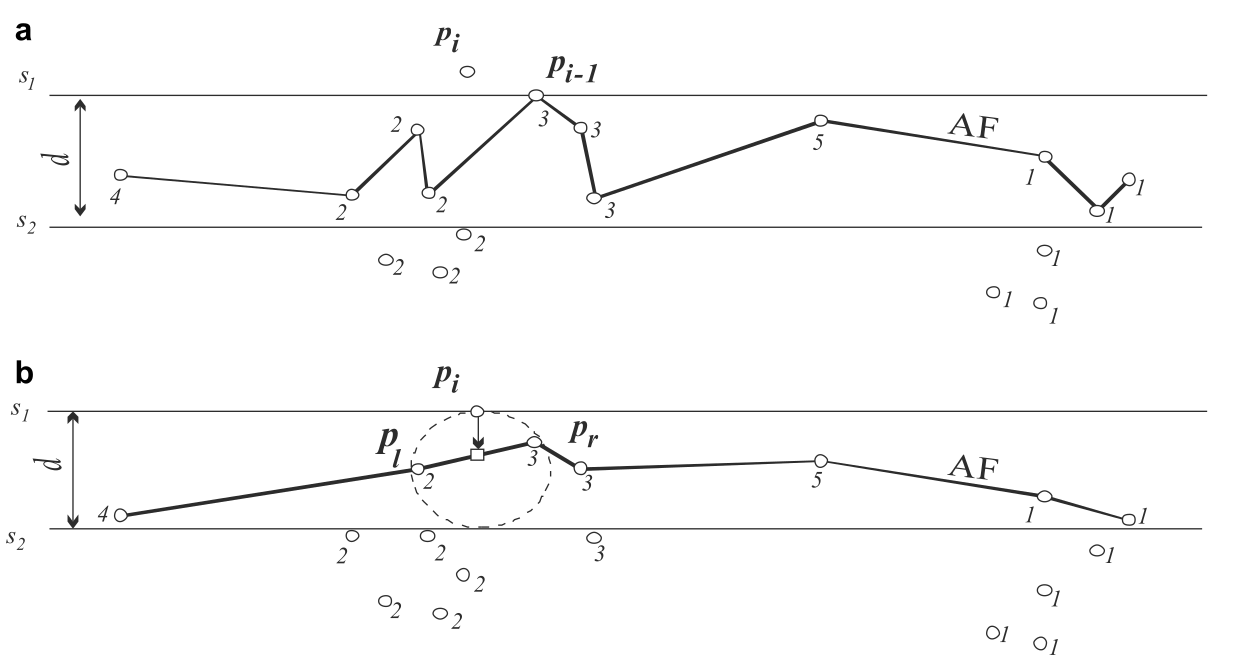
\includegraphics[width=\textwidth]{./Imagenes/Barrido.png}
      \caption*{i-ésima iteración.}
    \end{subfigure}
  \end{figure}
\end{frame}

\begin{frame}[fragile]{Algoritmo:}{Barrido II.}
  \begin{figure}
    \centering
    \begin{subfigure}[b]{0.6\textwidth}
      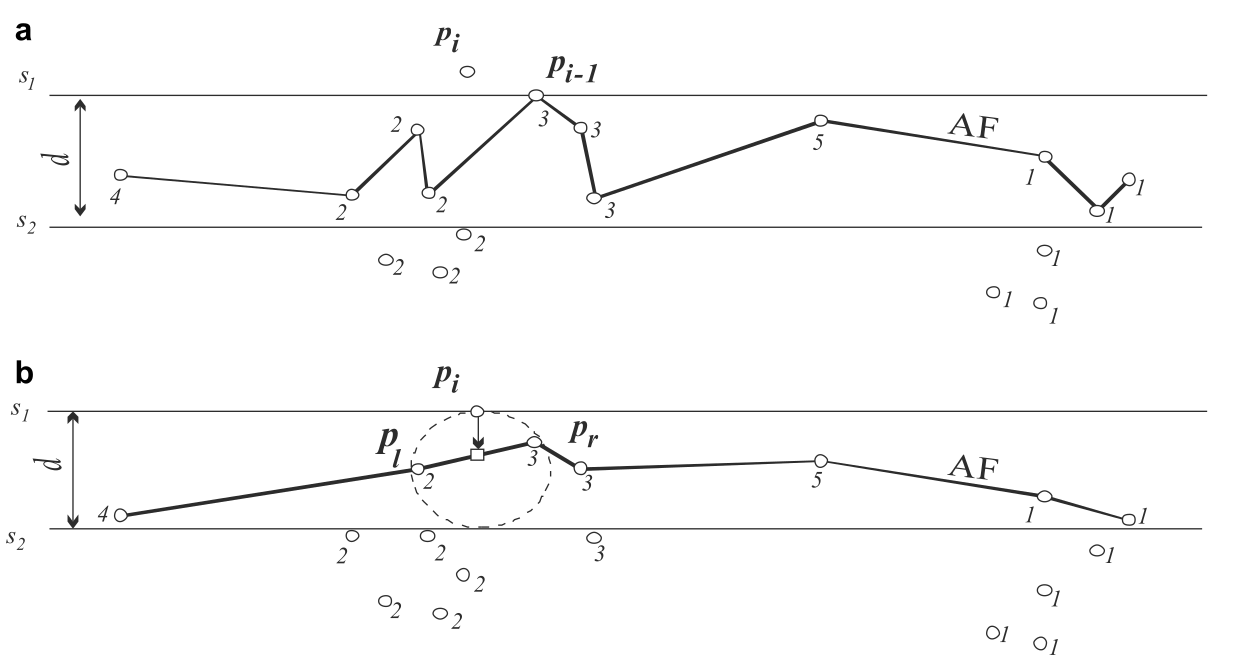
\includegraphics[width=\textwidth]{./Imagenes/Barrido.png}
      \caption*{i-ésima iteración.}
    \end{subfigure}
  \end{figure}
  \begin{enumerate}
  \item[4.] En la siguiente iteración $s_1$ se mueve al siguiente punto y $s_2$ la sigue
    a distancia $d$.
  \item[5.] Cuando un punto $p_i$ ingresa a la manga entre las líneas $s_1$ y $s_2$, se determina
    su proyección con AF. Entonces puede pasar que:
    \begin{enumerate}
    \item[5.1] La proyección alcanza el AF.
    \item[5.2] La proyección no alcanza el AF.
    \end{enumerate}
    \textbf{Obs.} Diremos que $d_l = ||p_i - p_l||$ y $d_l = ||p_i - p_r||.$
  \end{enumerate}
\end{frame}

\begin{frame}[fragile]{Algoritmo:}{Barrido III.}
  \begin{figure}
    \centering
    \begin{subfigure}[b]{0.6\textwidth}
      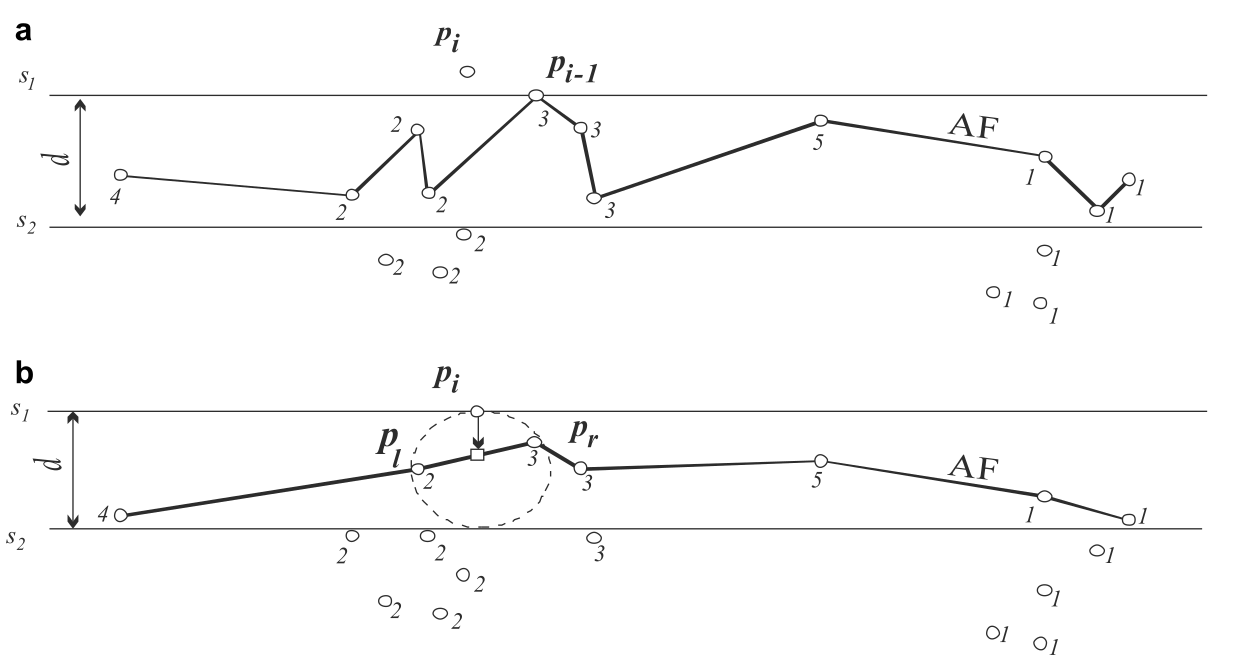
\includegraphics[width=\textwidth]{./Imagenes/Barrido.png}
      \caption*{i-ésima iteración.}
    \end{subfigure}
  \end{figure}
  \begin{enumerate}
  \item[5.1] La proyección alcanza el AF. Entonces, sucede que
    \begin{enumerate}
    \item[5.1.1] Si $d_l > d$ y $d_r > d$. Entonces, $p_i$ forma un nuevo grupo.
    \item[5.1.2] Si $d_l \leq d$ y $dr > d$. Entonces, $p_i$ forma parte del grupo de $p_l$.
    \item[5.1.3] Si $d_l > d$ y $dr \leq d$. Entonces, $p_i$ forma parte del grupo de $p_r$.
    \item[5.1.4] Si $d_l \leq d$ y $dr \leq d$. Entonces, $p_r, p_l, p_i$ forman un grupo.
    \end{enumerate}
  \item[5.2] La proyección no alcanza el AF. Se compara contra el último más cercano en AF, si
    no pertenece a ningún grupo existente forma uno nuevo.
    
    \textbf{Obs.} Diremos que $d_l = ||p_i - p_l||$ y $d_l = ||p_i - p_r||.$
  \end{enumerate}
\end{frame}
